\documentclass{standalone}

\usepackage{amsmath}

\usepackage{tikz}
\usetikzlibrary{backgrounds}
\usetikzlibrary{positioning}
\usetikzlibrary{calc}
\usetikzlibrary{trees}									% for trees
\usetikzlibrary{shapes.multipart}

\usepackage{xcolor}
\definecolor{mygreen}{RGB}{0,128,0}


\begin{document}
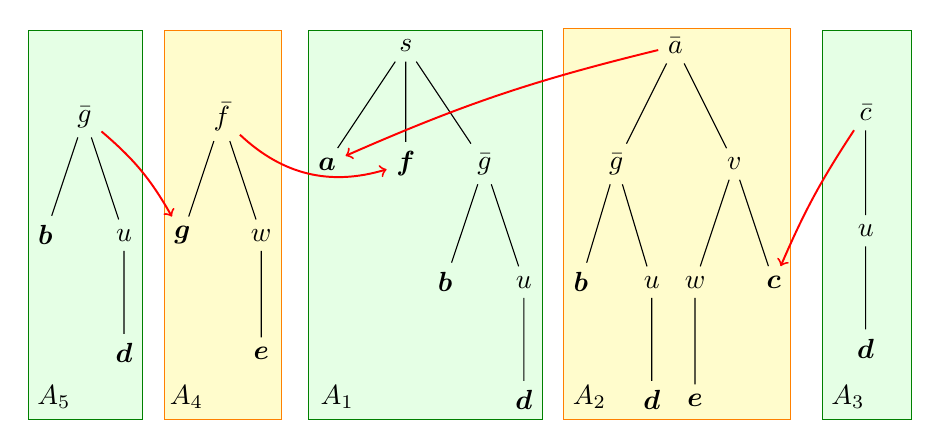
\begin{tikzpicture}



    %P: Argument for S
    \node (ps) {$s$}
    child {node[xshift=0.5cm] (pa) {$\boldsymbol{a}$}}
    child {node (pf) {$\boldsymbol{f}$}}
    child {node[xshift=-0.5cm]  (pxg) {$\bar{g}$}
            child {node[xshift=0.25cm]  (pb) {$\boldsymbol{b}$}}
            child {node[xshift=-0.25cm]  (pu) {$u$}
                    child { node (pd2) {$\boldsymbol{d}$} }
                }
        };

    \begin{pgfonlayer}{background}
        \filldraw [fill=green!20, fill opacity=0.5, draw=mygreen]
        (ps.north -| pa.west)
        rectangle (pd2.south -| pd2.east);
        \node at ([shift={(-3pt,8pt)}]pd2.south -| pa.east) {$A_1$};
    \end{pgfonlayer}

    % ------------------

    %O: Argument for xA
    \node[right = 3cm of ps] (pxa) {$\bar{a}$}
    child {node (pxaxg) {$\bar{g}$}
            child {node[xshift=0.3cm] (pxab) {$\boldsymbol{b}$}}
            child {node[xshift=-0.3cm] (pxau) {$u$}
                    child {node (pxad2) {$\boldsymbol{d}$}}
                }
        }
    child {node (pxav) {$v$}
            child { node[xshift=0.25cm] (pxaw) {$w$}
                    child { node (pxae) {$\boldsymbol{e}$} }
                }
            child { node[xshift=-0.25cm] (pxac) {$\boldsymbol{c}$} }
        };

    \begin{pgfonlayer}{background}
        \filldraw [fill=yellow!40, fill opacity=0.5, draw=orange]
        (pxa.north -| pxab.west)
        rectangle (pxad2.south -| pxac.east);

        \node at ([shift={(-3pt,8pt)}]pd2.south -| pxab.east) {$A_2$};
    \end{pgfonlayer}

    % ------------------

    %P: argument for xC    	
    \node[below right = 0.4cm and 2cm of pxa] (pxc) {$\bar{c}$}
    child {node (pxcu) {$u$}
            child {node (pxcd) {$\boldsymbol{d}$}}
        };

    \begin{pgfonlayer}{background}
        \filldraw [fill=green!20, fill opacity=0.5, draw=mygreen]
        ([shift={(-10pt,0pt)}] ps.north -| pxc.west)
        rectangle ([shift={(10pt,0pt)}]pd2.south -| pxcd.east);

        \node at ([shift={(-13pt,8pt)}]pd2.south -| pxcd.east) {$A_3$};
    \end{pgfonlayer}

    % ------------------

    % O: argument for xF    	

    \node[below left = 0.4cm and 1.9cm of ps] (pxf) {$\bar{f}$}
    child {node[xshift=0.25cm]  (pxfg) {$\boldsymbol{g}$}}
    child {node[xshift=-0.25cm]  (pxfw) {$w$}
            child { node (pxfe) {$\boldsymbol{e}$} }
        };

    \begin{pgfonlayer}{background}
        \filldraw [fill=yellow!40, fill opacity=0.5, draw=orange]
        (ps.north -| pxfg.west)
        rectangle (pd2.south -| pxfw.east);

        \node at ([shift={(-5pt,8pt)}]pd2.south -| pxfg.east) {$A_4$};
    \end{pgfonlayer}

    % ------------------

    % O: argument for xG    	

    \node[left = 1.3cm of pxf] (pxg2) {$\bar{g}$}
    child {node[xshift=0.25cm]  (pxg2b) {$\boldsymbol{b}$}}
    child {node[xshift=-0.25cm]  (pxg2u) {$u$}
            child { node (pxg2d) {$\boldsymbol{d}$} }
        };

    \begin{pgfonlayer}{background}
        \filldraw [fill=green!20, fill opacity=0.5, draw=mygreen]
        (ps.north -| pxg2b.west)
        rectangle (pd2.south -| pxg2d.east);
        \node at ([shift={(-3pt,8pt)}]pd2.south -| pxg2b.east) {$A_5$};
    \end{pgfonlayer}







    % \begin{pgfonlayer}{background}
    % \filldraw [fill=yellow!40]
    %               (xah.south -| xah.east)
    %     rectangle (xa.north -| xae.west);
    % \end{pgfonlayer}       

    % %O: Arg attacking A - 2		    
    % \node[right = 2cm of xa] (xa2) {$\bar{a}$}
    % child {node (xa2e) {$\boldsymbol{e}$}}
    % child {node (xa2v) {$v$}
    %     child {node (xa2i) {$\boldsymbol{i}$}}    
    % }; 

    % \begin{pgfonlayer}{background}
    % \filldraw [fill=yellow!40]
    %               (xa2i.south -| xa2i.east)
    %     rectangle (xa2.north -| xa2e.west);
    % \end{pgfonlayer}           

    % %O: Arg attacking A - 3				
    % \node[right = 1.25cm of xa2] (xa3) {$\bar{a}$}
    % child {node (xa3z) {$z$} 
    %     child {node (xa3f) {$\boldsymbol{f}$}}	
    % };

    % \begin{pgfonlayer}{background}
    % \filldraw [fill=yellow!40]
    %               (xa3f.south -| xa3f.east)
    %     rectangle (xa3.north -| xa3.west);
    % \end{pgfonlayer} 

    % %P: Arg attacking F					
    % \node[right = 0.4cm of xa3] (xf) {$\bar{f}$}
    % child {node (xfxe) {$\bar{e}$} 
    %     child {node (xfc) {$\boldsymbol{c}$}}	
    % };        

    % \begin{pgfonlayer}{background}
    % \filldraw[fill=green!10] %[top color=white, bottom color = green!20]
    %               (xfc.south -| xfc.east)
    %     rectangle (xf.north -| xf.west);
    % \end{pgfonlayer} 





    % attacks
    \path[->,draw,line width=0.25mm]
    (pxa) edge [bend right=5, red,] node {} (pa)
    (pxc) edge [bend right=5, red,] node {} (pxac)
    (pxf) edge [bend right=30, red,] node {} (pf)
    (pxg2) edge [bend left=10, red,] node {} (pxfg)
    ;
\end{tikzpicture}
\end{document}